\section{Architecture}
From the analysis of the project, it was clear that an OPC-UA
client was needed, as this should connect to the beer production machine. This
client should, in some way, store the collected data from the production machine,
which means that some kind of database should be a part of the MES. As the data
only consists of simple data types, integers, strings, etc., it is decided
to use a relational database. This way, data from different batches can easily
be stored in such a way that the relations between the data can be kept as
needed. By having a database, the subsystems do not have to store data
locally, thus making the same data available for other parts of the system,
securing data consistency. \\

It was discussed whether to develop a desktop client functioning as a dashboard
to control the production machine or if it should be a web client. A web client 
is chosen, as it is a more modern solution, it is more accessible than a desktop
client, as it can run in all supported web browsers and does not need to be
installed. If the company then chooses to change hardware, the dashboard is
still functional. \\

It was decided to develop a REST API, to make the data from the database
available to all subsystems in the MES. This API acts as a translator
between the subsystems in the MES, therefore simplifying the data management.
An example could be that the dashboard needs the data for a specific batch to
generate a batch report. Instead of having the dashboard communicate directly
with the database, a layer is added, the REST API, which both adds security and
handles the queries uniformly. The database then sends a query result to
the REST API, which then translates the SQL to JSON for the dashboard to read
and display to the user. \\

An overview of the MES to be developed can be seen in Figure
\ref{figure:architucture_diagram}.

\begin{figure}[ht]
	\centering 
	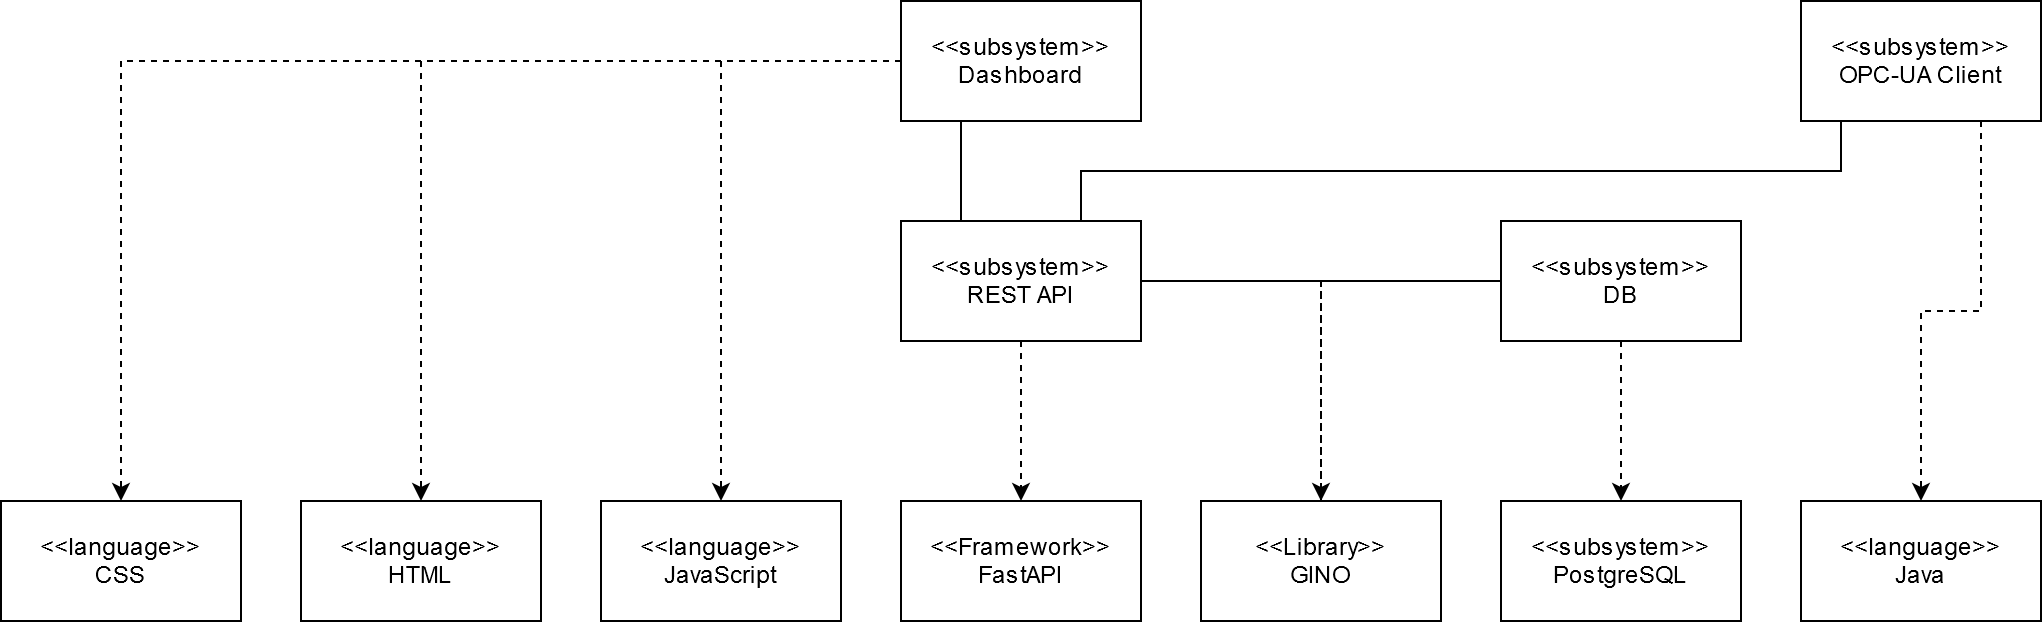
\includegraphics[width=1\textwidth]{images/diagrams/architecture_diagram.png}
	\caption{Software Architecture Diagram}
	\label{figure:architucture_diagram} 
\end{figure}
